%
% Main document
%

%
% Styles and packages
%

% !TEX root = ./main.tex

%\documentclass[10pt,a4paper]{report}
\documentclass[11pt,paper=a4,bibliography=totocnumbered,listof=numbered,DIV=calc,oneside,captions=tableheading,headinclude]{scrbook}
%footinclude

\usepackage[utf8]{inputenc}
\usepackage[left=2cm,right=2cm,top=2cm,bottom=2cm]{geometry}

\usepackage[swissgerman]{babel}

\usepackage{amsmath}
\usepackage{amsfonts}
\usepackage{amssymb}
\usepackage{array}
\usepackage{color}
\usepackage[T1]{fontenc}
\usepackage{float}
\usepackage{geometry}
\usepackage{graphicx}
\usepackage{helvet}
\usepackage{hyperref}
\usepackage{hyphsubst}
\usepackage{listings}
\usepackage{lmodern}
\usepackage{makeidx}
\usepackage[numbers]{natbib}
\usepackage{pdfpages}
\usepackage{qtree}
\usepackage{rotating}
\usepackage{tabularx}
\usepackage{url}
\usepackage{wallpaper}

% dev dependency
\usepackage{lipsum}


\begin{document}

  \title{Design von artifiziellen Tieren mit evolutionären Algorithmen}
  \author{Fabian Hediger \and Florian Tanner}
  \date{\today}

  \frontmatter

  %
% Cover page
%

% !TEX root = ./main.tex

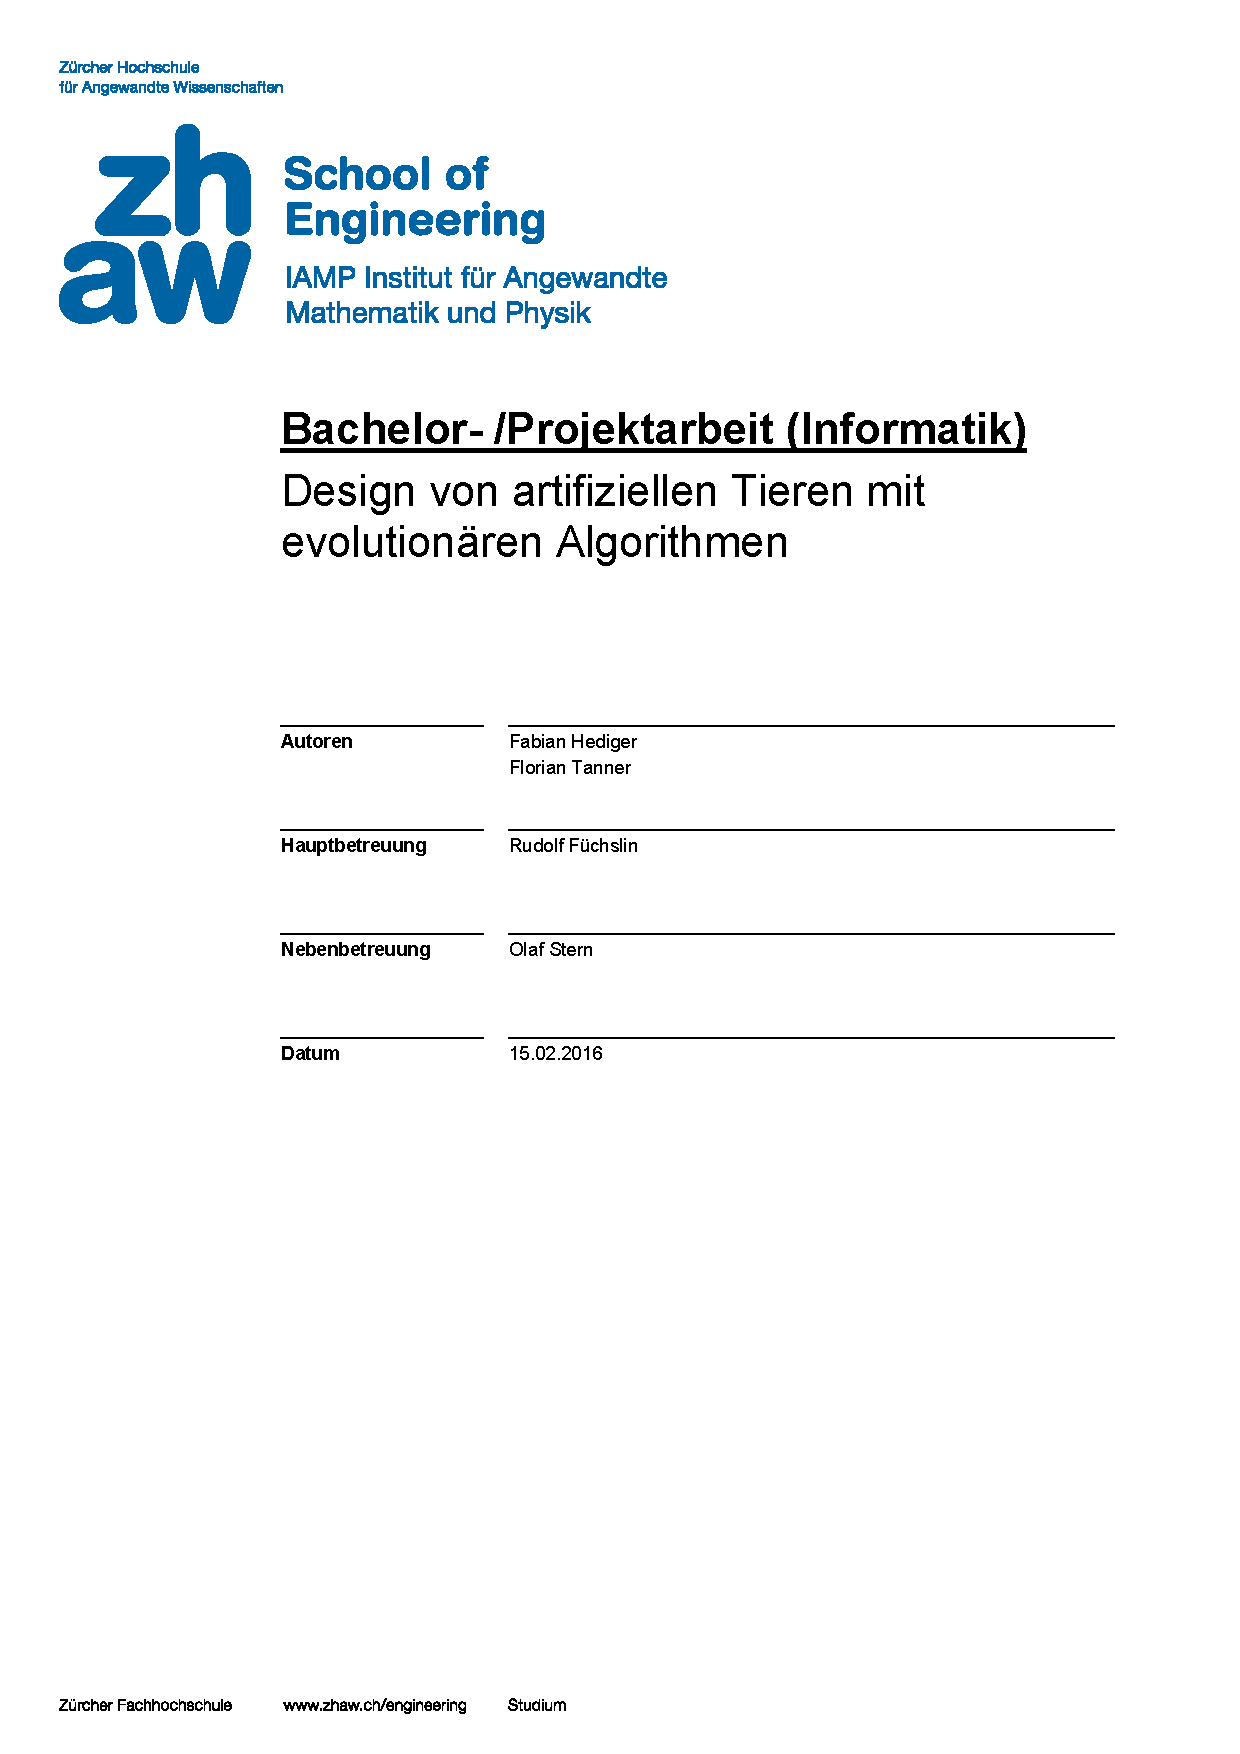
\includepdf{./SoE-IAMP_Bachelor-Titelblatt-Evolut.pdf}
\setcounter{page}{1}

  %
% Table of content
%

% !TEX root = ./main.tex

\tableofcontents
\newpage
\setcounter{page}{1}


  \chapter{Erklärung}
  \lipsum[1]

  \chapter{Vorwort}

    Natürliche Evolution hat kein vordefiniertes Ziel und ist ein sogennanter \grqq{} open-ended \grqq{} Anpassungsprozess. Artifizielle Evolution jedoch ist ein Optimierungsprozess, welcher versucht Lösungen zu vordefinierten Problem zu finden \cite{book:bioInspired}.


  \chapter{Abstract}
  \lipsum[3]

  \mainmatter

  \chapter{Einleitung}
  \lipsum[4-5]
  \section{Thema}
  \lipsum[5-6]

  \chapter{Theorie}
  \lipsum[6] \cite{IEEEexample:article_typical}
  \lipsum[7] \cite{mirrorcle_userguide}

  \chapter{Methode}
  \lipsum[8] \cite{microchip_spi} \cite{verryUseFulArticle}

  \chapter{Resultate}
  \lipsum[9]

  \appendix
  \chapter{Anhang}
  \section{Erster Anhang}

  \backmatter
  %
% Bibliography
%

% !TEX root = ./main.tex

\nobibliography*
\bibliographystyle{IEEEtranN}
\bibliography{IEEEabrv,literature}

  %
% Glossary entries
%

% !TEX root = ../main.tex

%
% Acronyms
%
\newacronym[see={FiniteStateMachine}]{fsm}{EA}{Endlicher Automat}

%
% Entries
%
\newglossaryentry{FiniteStateMachine}
{
  name={Endlicher Automat},
  description={Ein endlicher Automat (Zustandsmaschine, Zustandsautomat) ist ein Modell eines Verhaltens,
    bestehend aus Zuständen, Zustandsübergängen und Aktionen.}
}

\newglossaryentry{Hexapod}
{
  name={Hexapod},
  description={Die Sechsfüßer (griech. Hexapoda) oder Hexapoden
    gehören dem Stamm der Gliederfüßer (Arthropoda) an,
    sie bilden einen Unterstamm von diesen.}
}

\newglossaryentry{JointDriven}
{
  name={joint-driven},
  description={Ein Motor der ``joint-driven'' arbeitet steuert Bewegungen über ein Drehgelenk.
    }
}

\newglossaryentry{SimplePolygon}
{
  name={einfaches Polygon},
  description={Ein einfaches Polygon ist in der Geometrie eine flache Form bestehend aus geraden,
    sich nicht überschneidenden Linien, die einen geschlossenen Pfad formen.}
}


\end{document}
